\documentclass[10pt]{article}

\usepackage[spanish]{babel}
\usepackage{notasclase}
\usepackage{blindtext}
\usepackage{hyperref}
\usepackage{listings}
\usepackage{xcolor}
\definecolor{codegreen}{rgb}{0,0.6,0}
\definecolor{codegray}{rgb}{0.5,0.5,0.5}
\definecolor{codepurple}{rgb}{0.58,0,0.82}
\definecolor{backcolour}{rgb}{0.95,0.95,0.92}

\lstdefinestyle{mystyle}{
    backgroundcolor=\color{backcolour},
    commentstyle=\color{codegreen},
    keywordstyle=\color{magenta},
    numberstyle=\tiny\color{codegray},
    stringstyle=\color{codepurple},
    basicstyle=\ttfamily\footnotesize,
    breakatwhitespace=false,
    breaklines=true,
    captionpos=b,
    keepspaces=true,
    numbers=left,
    numbersep=5pt,
    showspaces=false,
    inputencoding=utf8,
    extendedchars=true,
    literate={á}{{\'a}}1 {é}{{\'e}}1 {í}{{\'i}}1 {ó}{{\'o}}1 {ú}{{\'u}}1 {Á}{{\'A}}1 {É}{{\'E}}1 {Í}{{\'I}}1 {Ó}{{\'O}}1 {Ú}{{\'U}}1 {ñ}{{\~n}}1 {Ñ}{{\~N}}1,
    showstringspaces=false,
    showtabs=false,
    tabsize=2
}


\lstset{style=mystyle}

\Titulo{Bases de Datos - TPI}

% Para debugear el estilo
\usepackage{lipsum}


\begin{document}

\begin{titlepage}
{
    \centering
    {\Large Licenciatura en Ciencia de Datos \par}
    {\bfseries\scshape\Large Escuela de Ciencia y Tecnología - UNSAM \par}
    \vspace{3cm}
    {\scshape\Huge Bases de Datos \par}
    {\itshape\Large Trabajo Práctico Integrador \par}
    \vfill
}
{\bfseries{\Large Profesores:}}

{\Large Laura Lazzati}

{\Large Rolando Titiosky}
\vspace{1cm}

{\bfseries{\Large Integrantes:}}

{\Large Gianni Bevilacqua}

{\Large Gerardo Toboso}

{\Large Javier Spina}

{\Large Bautista Turri}
\vfill
{\Large Junio 2025 \par}
\end{titlepage}

\section{Presentación del escenario}
\subsection{Empresa}
Una compañía tecnológica está desarrollando una plataforma integral basada en dispositivos portátiles inteligentes. Estas pulseras monitorean continuamente diversos parámetros biométricos relacionados con la salud y la actividad física de los usuarios. 
Los dispositivos capturan datos como: frecuencia cardíaca, calidad del sueño, niveles de actividad, entre otros. Además, se integran con una aplicación móvil que permite a los usuarios interactuar, visualizar información, recibir recomendaciones personalizadas y gestionar sus suscripciones.
Nosotros como equipo, estamos encargados del área de datos del proyecto. Nuestra metodología de trabajo está basada en Scrum, un tipo de metodología ágil que nos permite iterar sobre la implementación en ciclos de tiempo determinados. En una primera instancia, planeamos llegar a una versión MVP (minimum viable product: mínimo producto viable) para que la empresa analice resultados y pueda tomar decisiones informadas sobre el futuro del producto, y para poder cambiar aspectos clave del mismo y de los datos a consumir por las diferentes áreas.
\subsection{Situación a implementar}
El principal desafío es el diseño y desarrollo de una infraestructura de datos robusta y escalable, que pueda integrar y soportar múltiples fuentes de información. Por un lado, el sistema transaccional que gestiona las suscripciones, pagos y perfiles de usuarios. Por el otro, el flujo constante y masivo (en streaming) de los datos biométricos de los usuarios que se generan por el uso de las pulseras. También resulta fundamental incorporar la información de la interacción de los usuarios con la aplicación móvil: eventos de navegación, uso de funcionalidades, y comportamiento dentro de la plataforma.
\subsection{Justificación}
La solución que requiere la empresa implica unificar y consolidar toda la información detallada anteriormente en un Data Warehouse que funcione como el núcleo central de análisis de datos. Esto permite a la empresa obtener métricas clave y parámetros de desempeño del negocio, tales como tendencias de suscripción. Y tanto a la empresa como a los usuarios, les permite acceder a patrones de uso de las pulseras y la aplicación, así como indicadores de salud agregados.
Con esta implementación contamos con un modelo de datos integrado, que facilitará la generación de predicciones y modelos analíticos avanzados. Estos están orientados a optimizar la experiencia del usuario, mejorar la retención, detectar patrones de salud relevantes, y respaldar la toma de decisiones estratégicas a nivel comercial y operativo. De esta forma, establecemos una infraestructura capaz de soportar tanto análisis históricos como actuales, y la construcción de reportes y dashboards que reflejen el estado y evolución del negocio y la salud de sus usuarios.


\section{Presentación de los motores SQL y NoSQL}
\subsection{Proveedores}
Para el desarrollo del proyecto utilizamos los sistemas gestores de bases de datos Supabase (basado en PostgreSQL) y MongoDB Atlas (base de datos NoSQL), ambos ofrecidos como servicios en la nube.
\subsection{Justificar de las elecciones}
Optamos por estos motores debido a su facilidad de acceso y administración, al estar alojados en plataformas cloud que permiten la gestión remota de las bases de datos desde cualquier equipo con conexión a internet, eliminando la necesidad de contar con infraestructura física local (on-premise). Además, estas soluciones brindan escalabilidad y flexibilidad para manejar tanto datos estructurados (relacionales) como datos semi-estructurados o no estructurados, adaptándose así a los diferentes tipos de información que el proyecto requiere.
\subsection{Tipo de licencia}
Ambas plataformas ofrecen planes gratuitos que permiten comenzar el desarrollo sin costo inicial, ideal para el MVP. Tanto Supabase como MongoDB Atlas cuentan con opciones de suscripción pagas que proporcionan mayores recursos, capacidades y funcionalidades avanzadas, adecuándose a las necesidades de crecimiento del proyecto.
\subsection{Cómo conseguirlo, dónde descargarlo si se quiere hacer local}
Los servicios se pueden contratar y configurar directamente en sus portales oficiales:
\begin{itemize}
    \item \href{https://supabase.com/pricing}{Supabase - Planes y precios}
    \item \href{https://www.mongodb.com/pricing}{MongoDB Atlas - Planes y precios}
\end{itemize}
Para quienes deseen un entorno local, PostgreSQL puede descargarse e instalarse de forma gratuita desde su sitio oficial, mientras que MongoDB ofrece versiones Community para uso local disponibles en su portal.

\section{Diseño del Datawarehouse}
\subsection{Arquitectura BI}
La arquitectura de BI que implementamos para el proyecto sigue un esquema en capas basado en un proceso ETL (Extracción, Transformación y Carga), que permite consolidar y organizar datos provenientes de distintas fuentes operacionales.
\begin{itemize}
    \item {\bfseries Fuentes de datos}
    \begin{itemize}
        \item Una base de datos NoSQL (MongoDB Atlas) que almacena registros detallados y sin procesar de las actividades de los usuarios, recolectados tanto desde las pulseras inteligentes como desde la interacción con la aplicación móvil.
        \item Una base de datos relacional SQL (Supabase, basada en PostgreSQL) que gestiona información administrativa y transaccional, incluyendo datos de usuarios, planes, suscripciones y pagos.
    \end{itemize}
\item{\bfseries Proceso ETL} \par
Los datos se extraen de estas fuentes heterogéneas, luego se transforman para adecuarlos a las reglas del modelo dimensional definido, asegurando la calidad, coherencia y adecuación para análisis posteriores. Finalmente, los datos transformados se cargan en el Data Warehouse central, implementado sobre PostgreSQL en Supabase.
\item{\bfseries Uso posterior} \par
El Data Warehouse alimenta herramientas de visualización y reportes, facilitando la generación de dashboards con indicadores clave para el monitoreo y la toma de decisiones estratégicas del negocio.
\end{itemize}
\subsection{Motor seleccionado}
Para el Data Warehouse hemos elegido PostgreSQL, administrado mediante Supabase, debido a su combinación de robustez, escalabilidad y compatibilidad con operaciones analíticas complejas. Además, su integración con modernas herramientas de BI facilita la elaboración de reportes e informes detallados.




\subsection{Modelado de datos}
El diseño del Data Warehouse se basa en un esquema de modelo en {\bfseries estrella múltiple}, que combina varias tablas de hechos con sus correspondientes tablas de dimensiones
\begin{itemize}
    \item {\bfseries Tablas de hechos} \par
    \begin{itemize}
        \item \texttt{\bfseries hechos\_pagos}, que registra las transacciones relacionadas con la compra de planes y sus características cuantitativas.
        \item \texttt{\bfseries hechos\_actividad}, que almacena los registros de actividades realizadas por los usuarios a lo largo del tiempo.
    \end{itemize}


\item {\bfseries Tablas de dimensiones}\par

\begin{itemize}
    \item \texttt{dim\_usuario}, \texttt{dim\_fecha}, \texttt{dim\_plan}, \texttt{dim\_metodo\_pago}, \texttt{dim\_estado\_pago}, y \texttt{dim\_actividad}, que describen los atributos contextuales para el análisis de los hechos.
\end{itemize}
\end{itemize}
Este enfoque permite realizar análisis multidimensionales eficientes, facilitando el cruce de información desde diferentes perspectivas para obtener insights relevantes sobre el negocio y el comportamiento de los usuarios.

\subsection{Infraestructura usada: Diagramas y Máquinas}
\subsubsection{Diagramas elaborados}
\paragraph{Diagrama de flujo de datos }Representa visualmente el recorrido de la información desde sus fuentes originales (MongoDB y Supabase) hasta su consolidación en el Data Warehouse. Este diagrama facilita la comprensión del pipeline ETL y permite identificar puntos críticos en el proceso.

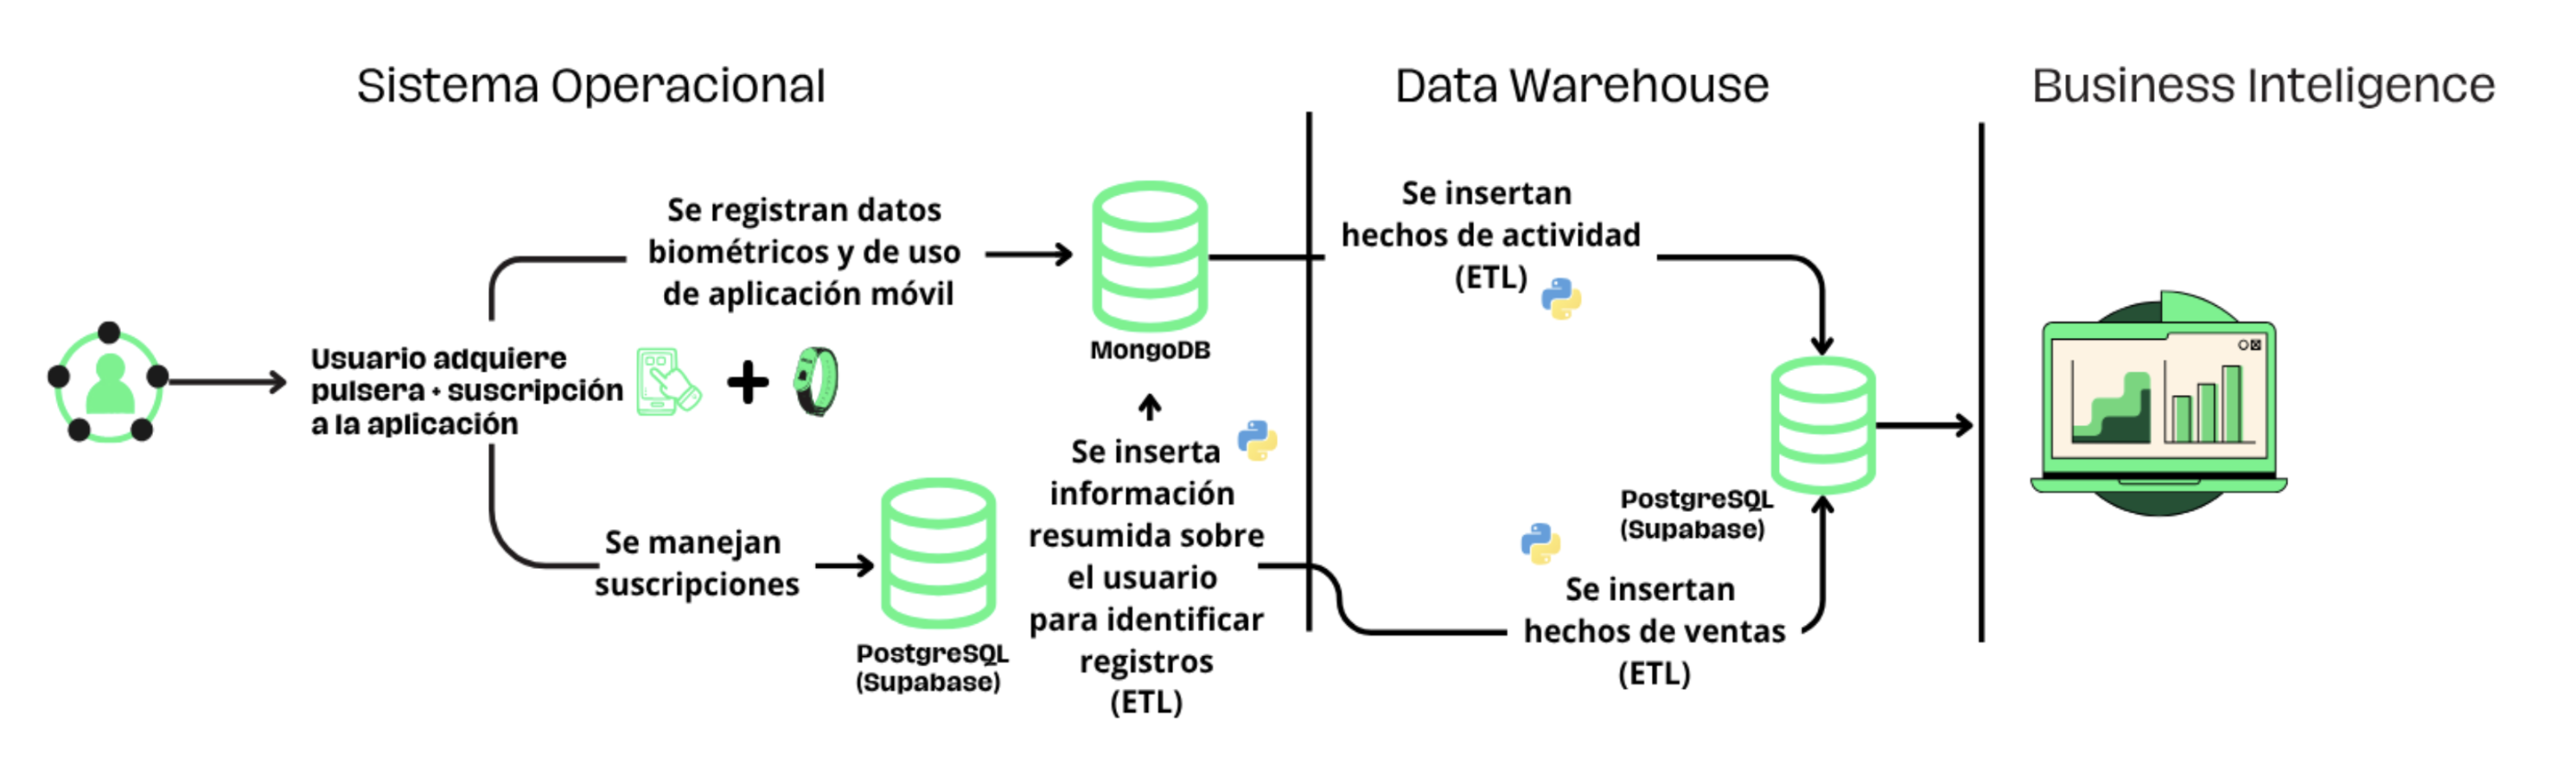
\includegraphics[width=0.95\textwidth]{img/flujo_datos.png}

\paragraph{Diagrama del modelo dimensional} Ilustra el esquema en estrella adoptado, mostrando las relaciones entre las tablas de hechos y las tablas de dimensiones. Este diagrama resulta esencial para entender la estructura del Data Warehouse y permite diseñar consultas analíticas eficientes.

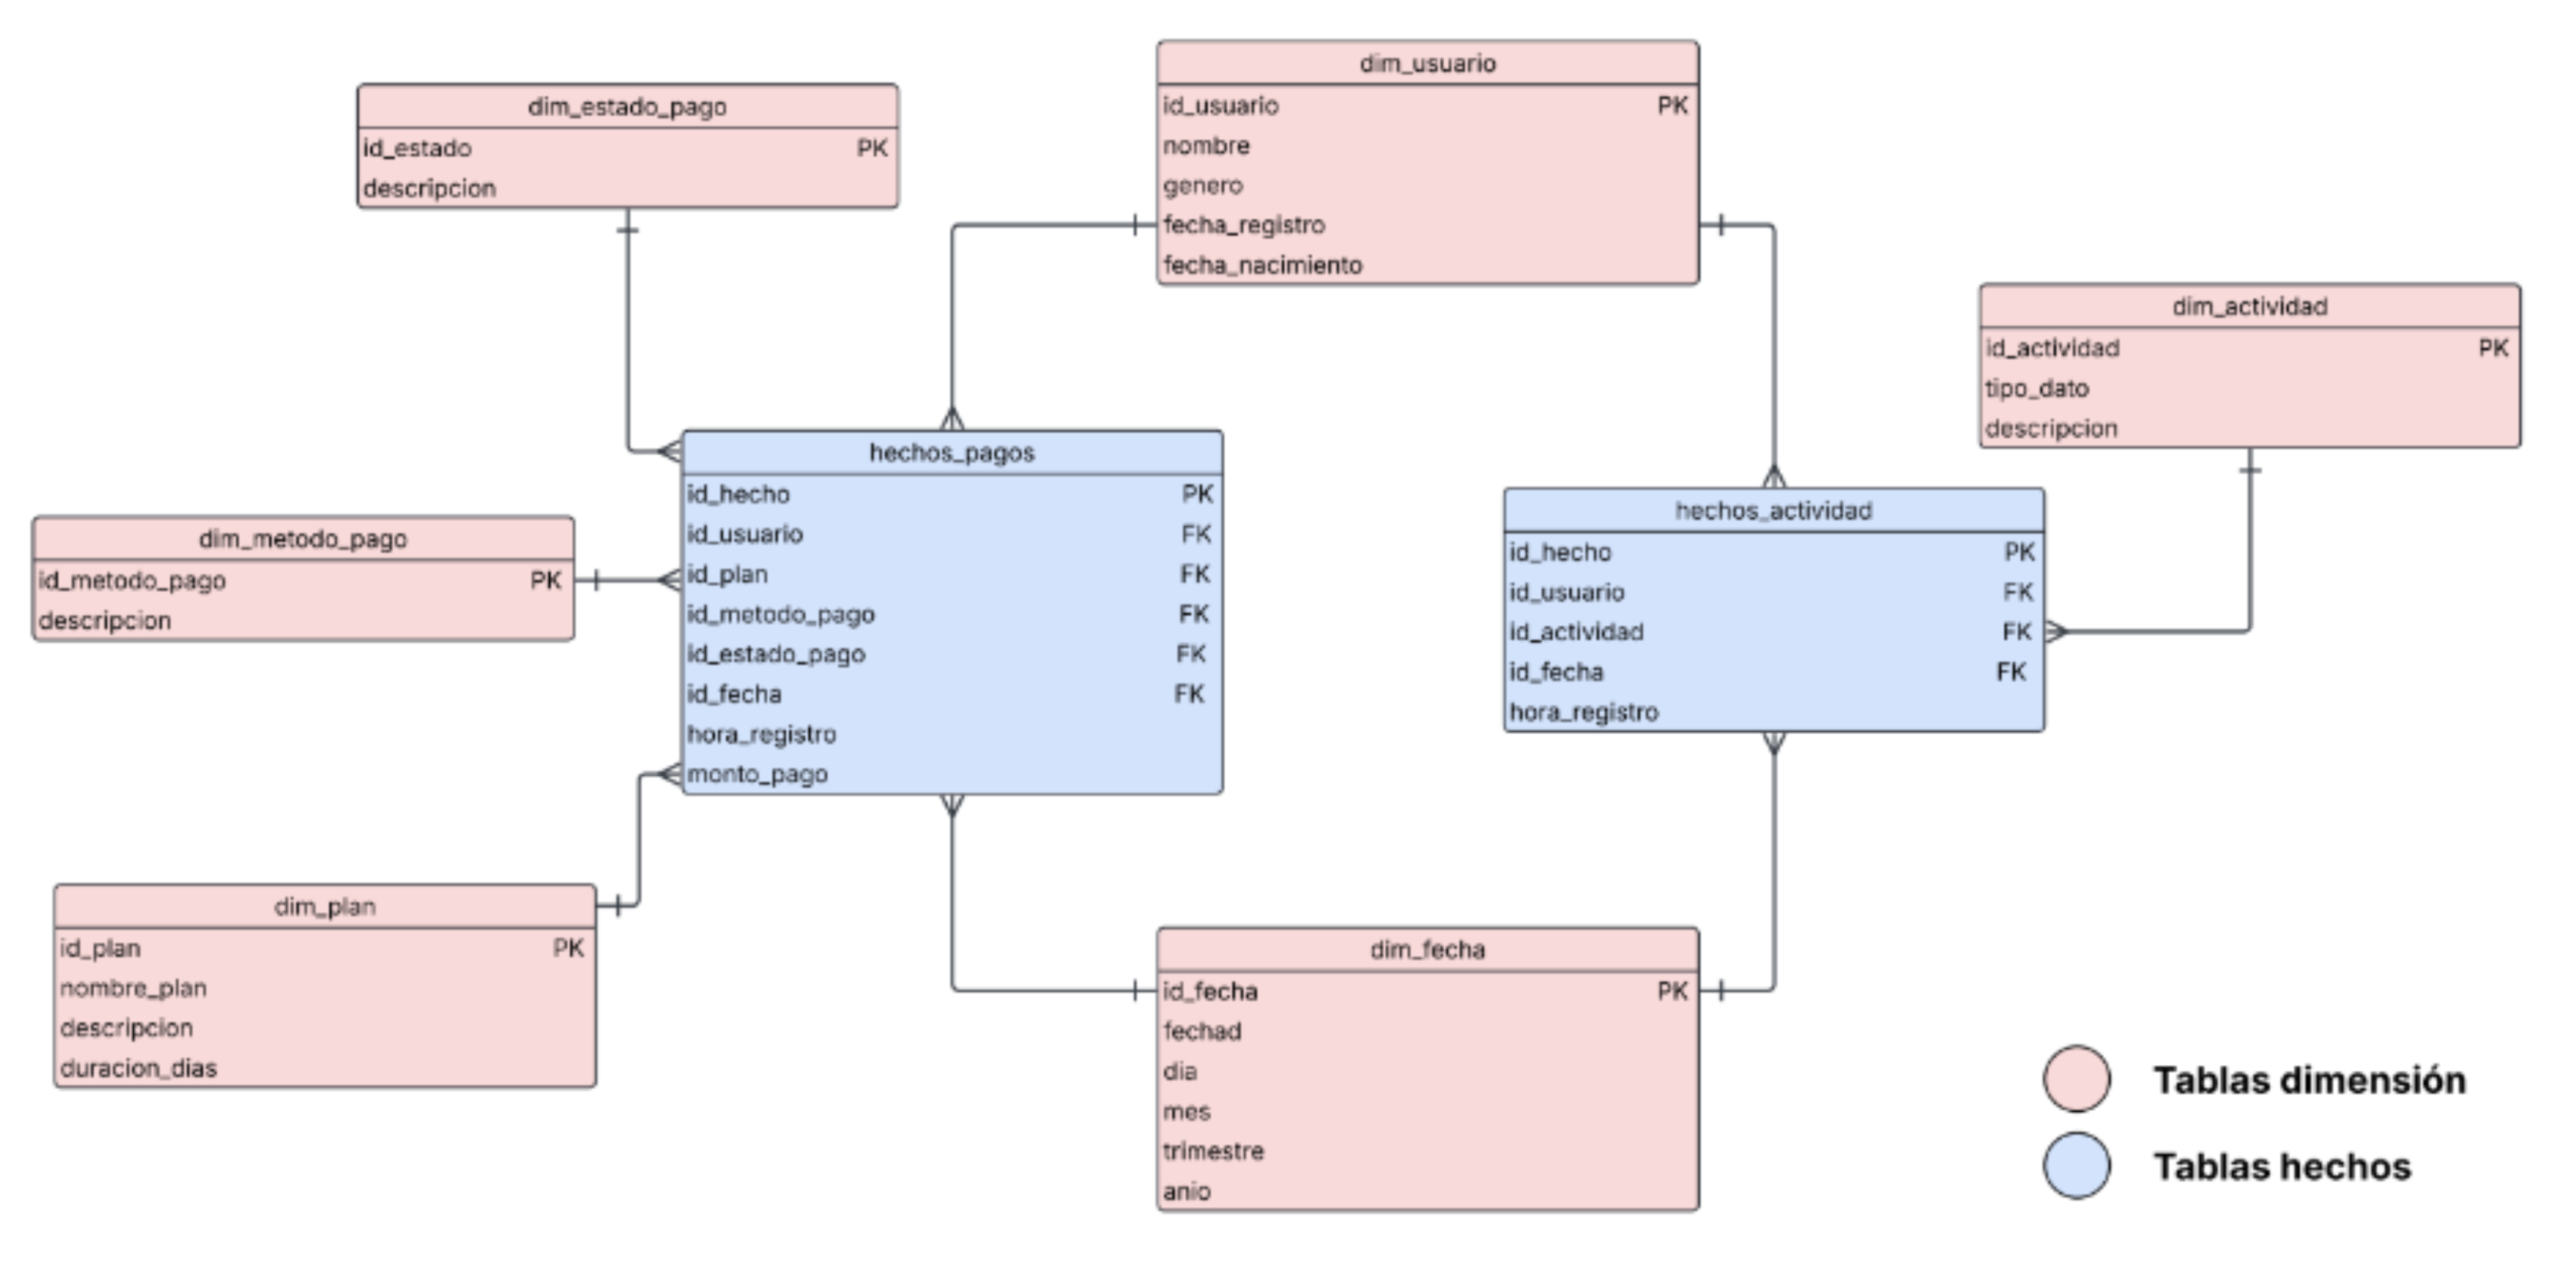
\includegraphics[width=0.9\textwidth]{img/modelo_dimensional.png}

\paragraph{Infraestructura tecnológica y estimación de recursos}
Luego de que las iteraciones pasen el estado de MVP, el volumen de datos provendrá de miles de usuarios que utilizarán simultáneamente las pulseras inteligentes y la aplicación móvil. De esta manera, se tendrá un flujo muy significativo de datos biométricos. La infraestructura deberá estar dimensionada para soportar esta carga sin perder rendimiento ni disponibilidad.
Para ello, seleccionamos servicios gestionados en la nube que sean escalables y balanceados entre las dimensiones de costos y prestaciones:
\begin{itemize}
    \item MongoDB Atlas (NoSQL): Para el almacenamiento de datos biométricos en formato JSON, se estima el uso de un clúster de nivel M20 o superior, que ofrece alrededor de 20 GB de almacenamiento y recursos computacionales suficientes para soportar escritura intensiva, consultas simultáneas y backups automáticos. Este tamaño permite absorber el volumen inicial esperado y crecer conforme aumente la base de usuarios y la frecuencia de recolección de datos.
    \item Supabase (PostgreSQL): Como base para el Data Warehouse y la gestión de datos estructurados de usuarios y suscripciones, se estima un plan con al menos 16 GB de almacenamiento, 4 vCPUs y 8 GB de RAM. Esta capacidad proporciona un rendimiento adecuado para cargas de trabajo analíticas y transaccionales, así como para la ejecución eficiente del pipeline ETL y la consulta de dashboards en tiempo real. De esta manera, la empresa podrá tener flexibilidad para ajustar recursos según la evolución del proyecto.
\end{itemize}





\section{Ejemplos de operaciones en el DW}

Presentamos las operaciones clave realizadas sobre el Data Warehouse, enfocadas en {\bfseries los usuarios}, ya que los consideramos el núcleo del sistema por su rol transversal en la generación de datos transaccionales y biométricos. Estas operaciones se ilustran con consultas y procesos relacionados con gestión de datos, particularmente sobre las tablas de hechos y dimensiones asociadas al comportamiento del usuario, como la tabla \texttt{dim\_usuario} y las tablas de hechos \texttt{hechos\_actividad} y \texttt{hechos\_pagos}.
\subsection{Creación}
Cuando un nuevo usuario se registra y contrata un plan a través del sistema transaccional, su información se almacena de forma estructurada en dicha base. Paralelamente, la información del usuario se guarda de forma resumida en la base de datos MongoDB (nombre, id y fecha de registro). Esto es para poder referenciar los registros que este genere posteriormente mediante el uso de la pulsera inteligente y la aplicación móvil.

\begin{lstlisting}[language=Python]
    def main():
    """
    Función principal que coordina el proceso ETL de carga de la dimensión de usuarios.
    """
    nombre_proceso = "ETL_CARGAR_DIM_USUARIO"

    with manejo_errores_proceso(nombre_proceso):
        # Conexiones a bases de datos
        db_transacciones = conectar_db_transacciones()
        db_dw = conectar_DW()

        # Verificación de la última fecha de inserción
        ultima_fecha_registro = extraer_ultima_fecha_insercion_dim_usuarios(db_dw)

        # Colocamos una fecha por defecto para la primera carga
        if not ultima_fecha_registro:
            ultima_fecha_registro = "2000-01-01T00:00:00Z"
            logger.info(f"Usando fecha por defecto para carga: {ultima_fecha_registro}")

        # Extracción de usuarios nuevos
        usuarios_nuevos = extraer_usuarios_por_fecha(db_transacciones, ultima_fecha_registro)

        # Inserción de usuarios en la dimensión
        if usuarios_nuevos:
            insertar_usuarios_dim(db_dw, usuarios_nuevos)
            logger.info(f"{nombre_proceso}: Proceso completado con éxito.")
        else:
            logger.info("No hay usuarios nuevos para insertar en la dimensión.")

\end{lstlisting}

Luego, cada cierto periodo de tiempo, se ejecuta un proceso de integración que forma parte del pipeline ETL. El objetivo es:

\paragraph{Extraer} nuevos registros de usuarios desde la base de datos transaccional.

\begin{lstlisting}[language=Python]
    def extraer_ultima_fecha_insercion_dim_usuarios(db_dw):
    """
    Obtiene la fecha del último registro insertado en la tabla de dimensión de usuarios.
    
    Args:
        db_dw: Conexión a la base de datos.
        
    Returns:
        str: Fecha del último registro o None si no hay registros.
    """
    try:
        respuesta = (
            db_dw.table("dim_usuario")
            .select("fecha_registro")
            .order("fecha_registro", desc=True)
            .limit(1)
            .execute()
        )
        
        if not respuesta.data:
            logger.info("No existen registros previos en la dimensión de usuarios.")
            return None
            
        ultima_fecha = respuesta.data[0]["fecha_registro"]
        logger.info(f"Última fecha de inserción en dimensión usuarios: {ultima_fecha}")
        return ultima_fecha
    except Exception as e:
        logger.error(f"Error al extraer última fecha de inserción en dim_usuario: {e}")
        raise
\end{lstlisting}

\begin{lstlisting}[language=Python]
    def extraer_usuarios_por_fecha(db_transacciones, fecha_registro):
    """
    Extrae usuarios de la base de datos operacional que fueron registrados
    después de la fecha especificada.
    
    Args:
        db_transacciones: Conexión a la base de datos operacional.
        fecha_registro (str): Fecha de registro a partir de la cual extraer usuarios.
        
    Returns:
        list: Lista de diccionarios con datos de usuarios.
    """
    try:
        respuesta = (
            db_transacciones.table("usuarios")
            .select(
                """
                id_usuario,
                nombre,
                genero:genero(genero),
                fecha_registro,
                fecha_nacimiento
                """
            )
            .gt("fecha_registro", fecha_registro)
            .execute()
        )
        
        usuarios = respuesta.data
        logger.info(f"Extraídos {len(usuarios)} usuarios nuevos desde la base operacional.")
        return usuarios
    except Exception as e:
        logger.error(f"Error al extraer usuarios por fecha: {e}")
        raise
\end{lstlisting}

\paragraph{Cargar} los registros depurados en la tabla \texttt{dim\_usuario} del Data Warehouse, donde el registro correspondiente queda preparado para poder {\bfseries relacionarlo con hechos} que luego el usuario genere.

\begin{lstlisting}[language=Python]
    def insertar_usuarios_dim(db_dw, usuarios):
    """
    Inserta usuarios en la dimensión de usuarios de la base de datos dimensional.
    
    Args:
        db_dw: Conexión a la base de datos.
        usuarios (list): Lista de diccionarios con datos de usuarios a insertar.
        
    Returns:
        int: Número de usuarios insertados correctamente.
    """
    contador_exito = 0
    contador_error = 0
    
    for usuario in usuarios:
        try:
            db_dw.table("dim_usuario").insert(
                {
                    "id_usuario": usuario["id_usuario"],
                    "nombre": usuario["nombre"],
                    "genero": usuario["genero"]["genero"],
                    "fecha_registro": usuario["fecha_registro"],
                    "fecha_nacimiento": usuario["fecha_nacimiento"],
                }
            ).execute()
            logger.info(f"Usuario {usuario['nombre']} (ID: {usuario['id_usuario']}) insertado en dim_usuario.")
            contador_exito += 1
        except Exception as e:
            logger.error(f"Error al insertar usuario {usuario['nombre']} (ID: {usuario['id_usuario']}) en dim_usuario: {e}")
            contador_error += 1
    
    logger.info(f"Dimensión Usuarios: {contador_exito} usuarios insertados, {contador_error} errores.")
    return contador_exito
\end{lstlisting}

Este flujo garantiza que la dimensión de usuarios se mantenga actualizada y alineada con las fuentes operativas, permitiendo obtener indicadores como la evolución del número de usuarios activos, la distribución por tipo de plan, o algún otro tipo de segmentación.

\subsection{Eliminación}
En este sistema no se eliminan registros de forma definitiva con fines históricos y analíticos, salvo excepciones. En lugar de eliminar físicamente los registros de usuarios, se emplea una política de {\bfseries borrado lógico} mediante el análisis de suscripciones activas por parte de los usuarios, que indica si el usuario sigue activo, se ha dado de baja o presenta un estado inactivo. Esta estrategia permite conservar el historial completo de interacciones y mantener la integridad de los análisis longitudinales, como el cálculo de tasas de retención o el análisis del ciclo de vida del cliente.

Dentro de las excepciones, contamos el borrado por motivos de cumplimiento de normativas vigentes y cumplimiento de lo acordado entre cada usuario y la empresa por medio de los Términos y Condiciones del uso de la pulsera (a delimitar por el equipo Legal de la empresa). Las normativas que podemos tener en cuenta son, por ejemplo, la Ley de Protección de Datos Personales en Argentina (Ley 25.326), GDPR en Europa y el CCPA en California, Estados Unidos. Además, por motivos de límite en las suscripciones activas a las bases de datos, se puede proceder a la eliminación de información, pero todo esto está fuera del alcance del MVP. Sugerimos implementar a futuro los métodos que guardaran información anonimizada y agregada del uso de las pulseras y la aplicación.
\subsection{Inserción}
\subsubsection{Contexto y flujo ETL}
Una vez que un usuario ha sido registrado en la dimensión \texttt{dim\_usuario} del Data Warehouse y ha comenzado a interactuar con la aplicación y la pulsera inteligente, se genera un flujo constante de datos biométricos (como actividad física, sueño o niveles de glucosa) y de uso de la aplicación móvil. Esta información se almacena inicialmente en la base de datos MongoDB, en formato semiestructurado.

\begin{lstlisting}
    _id: ObjectId('6838bf11a14861129921861a')
    id_usuario: 1
    tipo_registro: "actividad"
    timestamp: "2025-05-29T08:21:53.508+00:00"
    datos:
        tipo_actividad: "correr"
        duracion_min: 119
        distancia_km: 11.9
        pasos: 13622
        calorias_quemadas: 176
        repeticiones: null
        peso_levantado_kg: null
        ritmo_cardiaco_prom: 136

\end{lstlisting}

\begin{lstlisting}[language=Python]
    def main():
    """
    Función principal que coordina el proceso ETL de carga de hechos de actividad.
    """
    nombre_proceso = "ETL_CARGAR_HECHOS_ACTIVIDAD"
    
    with manejo_errores_proceso(nombre_proceso):
        # Conexiones a bases de datos
        db_sensor_pulsera = conectar_db_sensor_pulsera()
        db_dw = conectar_DW()
        
        try:
            # Obtención de usuarios
            usuarios = list(db_sensor_pulsera.pulseras_inteligentes.usuarios_sensor.find())
            
            # Obtención de la última fecha de carga
            ultima_fecha_transaccion = extraer_ultima_fecha_insercion_hechos(db_dw, 'hechos_actividad')
            
            # Fecha por defecto para primera carga
            if not ultima_fecha_transaccion:
                ultima_fecha_transaccion = "2000-01-01T00:00:00Z"
                logger.info(f"Usando fecha por defecto para primera carga: {ultima_fecha_transaccion}")
            
            # Conversión a formato datetime para compatibilidad con mongo
            if isinstance(ultima_fecha_transaccion, str):
                try:
                    ultima_fecha_transaccion = datetime.fromisoformat(ultima_fecha_transaccion.replace("Z", "+00:00"))
                except Exception as e:
                    logger.error(f"Error convirtiendo fecha: {e}")
            
            # Contadores para el resumen
            total_actividad_fisica = 0
            total_actividad_aplicacion = 0
            
            # Procesamiento por usuario
            for usuario in usuarios:
                id_usuario = usuario["id_usuario"]
                
                # Procesamiento de actividad física
                actividades_fisicas = extraer_actividad_fisica(db_sensor_pulsera, id_usuario, ultima_fecha_transaccion)
                registros_act_fisica = procesar_actividades_fisicas(db_dw, actividades_fisicas, id_usuario)
                total_actividad_fisica += registros_act_fisica
                
                # Procesamiento de uso de aplicación
                actividades_aplicacion = extraer_actividad_aplicacion(db_sensor_pulsera, id_usuario, ultima_fecha_transaccion)
                registros_act_aplicacion = procesar_actividades_aplicacion(db_dw, actividades_aplicacion, id_usuario)
                total_actividad_aplicacion += registros_act_aplicacion
            
            # Resumen final
            logger.info(f"Carga completada: {total_actividad_fisica} registros de actividad física, " 
                        f"{total_actividad_aplicacion} registros de actividad de aplicación")
        finally:
            # Cierre de conexiones
            db_sensor_pulsera.close()
\end{lstlisting}

Con frecuencia periódica, se ejecuta un proceso ETL que {\bfseries extrae} los registros recientes desde MongoDB, filtrando por eventos biométricos y de interacción relevantes.

\begin{lstlisting}[language=Python]
    def extraer_actividad_fisica(db_sensor_pulsera, id_usuario, fecha_base):
    """
    Extrae registros de actividad física para un usuario desde MongoDB,
    posteriores a una fecha determinada.
    
    Args:
        db_sensor_pulsera: Conexión a la base de datos MongoDB.
        id_usuario (int): ID del usuario.
        fecha_base (datetime): Fecha a partir de la cual extraer registros.
        
    Returns:
        list: Lista de documentos con datos de actividad física.
    """
    try:
        datos_db_sensor = db_sensor_pulsera.pulseras_inteligentes.datos_sensor
        
        actividades = list(datos_db_sensor.find({
            "id_usuario": id_usuario,
            "tipo_registro": "actividad", 
            "timestamp": {"$gt": fecha_base}
        }))
        
        logger.debug(f"Extraídos {len(actividades)} registros de actividad física para usuario {id_usuario}")
        return actividades
    except Exception as e:
        logger.error(f"Error al extraer actividad física para usuario {id_usuario}: {e}")
        return []
\end{lstlisting}

\begin{lstlisting}[language=Python]
    def extraer_actividad_aplicacion(db_sensor_pulsera, id_usuario, fecha_base):
    """
    Extrae registros de uso de aplicación para un usuario desde MongoDB,
    posteriores a una fecha determinada.
    
    Args:
        db_sensor_pulsera: Conexión a la base de datos MongoDB.
        id_usuario (int): ID del usuario.
        fecha_base (datetime): Fecha a partir de la cual extraer registros.
        
    Returns:
        list: Lista de documentos con datos de uso de aplicación.
    """
    try:
        datos_db_aplicacion = db_sensor_pulsera.pulseras_inteligentes.datos_aplicacion
        
        actividades = list(datos_db_aplicacion.find({
            "id_usuario": id_usuario,
            "timestamp": {"$gt": fecha_base}
        }))
        
        logger.debug(f"Extraídos {len(actividades)} registros de actividad de aplicación para usuario {id_usuario}")
        return actividades
    except Exception as e:
        logger.error(f"Error al extraer actividad de aplicación para usuario {id_usuario}: {e}")
        return []
\end{lstlisting}

\paragraph{Transforma} los datos, mapeando los atributos de actividad y de tiempo a los identificadores definidos en el modelo dimensional (por ejemplo, \texttt{id\_usuario}, \texttt{id\_actividad} e \texttt{id\_fecha}), y normalizando los formatos según el esquema del Data Warehouse.

\begin{lstlisting}[language=Python]
    def procesar_actividades_fisicas(db_dw, actividades, id_usuario):
    """
    Procesa y carga registros de actividad física en la tabla de hechos.
    
    Args:
        db_dw: Conexión al Data Warehouse.
        actividades (list): Lista de documentos con datos de actividad física.
        id_usuario (int): ID del usuario.
        
    Returns:
        int: Número de registros insertados correctamente.
    """
    contador = 0
    
    for actividad in actividades:
        # Nombre e ID de la actividad
        nombre_actividad = actividad["datos"]["tipo_actividad"]
        id_actividad = obtener_id_actividad(db_dw, nombre_actividad)
        
        # ID de fecha y hora de la actividad
        id_fecha = obtener_id_fecha(db_dw, actividad["timestamp"])
        hora_actividad = extraer_hora_fecha(actividad["timestamp"])
        
        # Inserción del hecho
        if insertar_hecho_actividad(db_dw, id_usuario, id_actividad, id_fecha, hora_actividad):
            contador += 1
    
    return contador
\end{lstlisting}

\begin{lstlisting}[language=Python]
    def procesar_actividades_aplicacion(db_dw, actividades, id_usuario):
    """
    Procesa y carga registros de uso de aplicación en la tabla de hechos.
    
    Args:
        db_dw: Conexión al Data Warehouse.
        actividades (list): Lista de documentos con datos de uso de aplicación.
        id_usuario (int): ID del usuario.
        
    Returns:
        int: Número de registros insertados correctamente.
    """
    contador = 0
    
    for actividad in actividades:
        # Nombre e ID de la actividad
        nombre_actividad = actividad["tipo_evento"]
        id_actividad = obtener_id_actividad(db_dw, nombre_actividad)
        
        # ID de fecha y hora de la actividad
        id_fecha = obtener_id_fecha(db_dw, actividad["timestamp"])
        hora_actividad = extraer_hora_fecha(actividad["timestamp"])
        
        # Inserción del hecho
        if insertar_hecho_actividad(db_dw, id_usuario, id_actividad, id_fecha, hora_actividad):
            contador += 1
    
    return contador

\end{lstlisting}

\paragraph{Carga} la información procesada en la tabla de hechos: \texttt{hechos\_actividad}.

\begin{lstlisting}[language=Python]
    def insertar_hecho_actividad(db_dw, id_usuario, id_actividad, id_fecha, hora_registro):
    """
    Inserta un registro en la tabla de hechos de actividad.
    
    Args:
        db_dw: Conexión al Data Warehouse.
        id_usuario (int): ID del usuario.
        id_actividad (int): ID de la actividad.
        id_fecha (int): ID de la fecha.
        hora_registro (str): Hora del registro en formato HH:MM:SS.
        
    Returns:
        bool: True si la inserción fue exitosa, False en caso contrario.
    """
    try:
        if not all([id_usuario, id_actividad, id_fecha, hora_registro]):
            logger.warning(f"Datos incompletos para inserción: usuario={id_usuario}, actividad={id_actividad}, fecha={id_fecha}")
            return False
            
        db_dw.table("hechos_actividad").insert({
            "id_usuario": id_usuario,
            "id_actividad": id_actividad,
            "id_fecha": id_fecha,
            "hora_registro": hora_registro
        }).execute()
        
        logger.debug(f"Hecho insertado: usuario={id_usuario}, actividad={id_actividad}, fecha={id_fecha}")
        return True
    except Exception as e:
        logger.error(f"Error al insertar hecho para usuario {id_usuario}: {e}")
        return False
\end{lstlisting}

Para el caso particular que tomamos al principio podemos ver el resultado de este proceso ETL

\begin{lstlisting}[language=sql]
    SELECT *
    FROM hechos_actividad
    WHERE
        id_usuario = 1 AND
        id_actividad = 6 AND
        id_fecha = 149;

    +-----------+-------------+---------------+-----------+----------------+
    | id_hecho  | id_usuario  | id_actividad  | id_fecha  | hora_registro  |
    +-----------+-------------+---------------+-----------+----------------+
    |        1  |          1  |            6  |       149 |       08:21:53 |
    +-----------+-------------+---------------+-----------+----------------+
\end{lstlisting}

Cada registro de hechos mantiene integridad referencial con las dimensiones correspondientes, especialmente \texttt{dim\_usuario}, permitiendo realizar análisis cruzados entre comportamientos y atributos del usuario.
\paragraph{Validación de integridad}
El proceso ETL incluye controles que aseguran que los registros solo se inserten si el usuario asociado ya se encuentra registrado en la dimensión correspondiente. Esto previene inconsistencias y garantiza la confiabilidad de los datos analíticos generados a partir del Data Warehouse.

\end{document}